\documentclass[letter, 10pt]{article}

\usepackage{xcolor}
\usepackage{subfig}
\usepackage[margin = 1in]{geometry}
\usepackage{graphicx}
\usepackage{epstopdf}
\usepackage{pxfonts}
\usepackage{setspace}
\usepackage{titlesec}
\usepackage{booktabs}
\usepackage{fancyhdr}
\usepackage{listings}
\usepackage{multirow}
\usepackage{tikz}
\usepackage{ragged2e}
\usetikzlibrary{positioning}
\usetikzlibrary{fit}

\definecolor{evolotus-color}{RGB}{56,64,96}

\titlespacing{\section}{0pt}{\baselineskip}{0.5\baselineskip}
\titleformat{\section}{\normalfont\fontsize{14}{0}\bfseries}{\thesection}{1em}{}
\titlespacing{\subsection}{0pt}{\baselineskip}{0.2\baselineskip}
\titleformat{\subsection}{\normalfont\fontsize{12}{0}\bfseries}{\thesubsection}{1em}{}

\def\helv{\fontfamily{phv}\bfseries\selectfont}

\begin{document}
\begin{onehalfspacing}

{\noindent\Large\uppercase{16-662 Robot Autonomy}\\[8pt]
{\Huge PROJECT 1A: REPORT}}\\[4pt]

{\noindent\scriptsize Team Evolutus \\[-0.5\baselineskip]
\noindent\scriptsize William Ku ({\tt wku}), Yuhan Long ({\tt yuhanlon}), Yu-Te Cheng ({\tt yutec}), Dawei Wang ({\tt daweiwan}).} 
	
\noindent\today

\pagestyle{fancy}
\lhead{Project 1A}
\rhead{Team Evolutus}

\setlength{\parskip}{0.5\baselineskip}
\RaggedRight
\parindent=2em

\section{System Diagram}

Figure \ref{matlab-quadrotor-interface} displays the system diagram of the
software pipeline ({\tt simple\_io\_test.m}).

\tikzstyle{node} = [draw, rounded corners, thick, inner sep = 6pt, align = left]
\tikzstyle{topic} = [fill = gray!20, font = \tt\scriptsize, inner sep = 2pt, text width = 1.5cm]

\tikzstyle{dir} = [rounded corners = 2pt, text = white, inner sep = 3pt, font = \helv\scriptsize]
\tikzstyle{din} = [dir, fill = red!40!black]
\tikzstyle{dout} = [dir, fill = blue!40!black]

\begin{figure}[h!]
	\centering
	
	\begin{tikzpicture}[node distance = 2pt]
	
		\matrix [anchor = west, text depth = 0pt, row sep = 4pt, column sep = 4pt, align = left] (mat) {		
			\node (odompub) {Odometry \\ \tt odom\_pub}; & \node (odomout) [dout] {\scriptsize\helv OUT}; & \node [text width = 4cm] {};
				& \node (ipcodom) [align = left, inner sep = 6pt, draw, rounded corners, fill = red!10]
					{\tt /alpha/matlab\_odom \\ (ipc\_bridge)}; & \node [text width = 0.5cm] {};
				& \node (odomin) [din] {\scriptsize\helv IN}; & \node (odomsub) {Odometry \\ \tt odom\_sub}; \\			
			\node (imupub) {IMU \\ \tt imu\_pub}; & \node (imuout) [dout] {\scriptsize\helv OUT}; &
				& \node (ipcimu) [align = left, inner sep = 6pt, draw, rounded corners, fill = red!10]
					{\tt /alpha/matlab\_imu \\ (ipc\_bridge)}; &
				& \node (imuin) [din] {\helv\scriptsize IN}; & \node (imusub) {IMU \\ \tt imu\_sub}; \\
			\node (cmdsub) {Command \\ \tt cmd\_sub}; & \node (cmdin) [din] {\helv\scriptsize IN}; &
				& \node (ipccmd) [align = left, inner sep = 6pt, draw, rounded corners, fill = red!10]
					{\tt /alpha/matlab\_pd \\ (quadrotor\_msgs)}; &
				& \node (cmdout) [dout] {\helv\scriptsize OUT}; & \node (cmdpub) {Command \\ \tt cmd\_pub}; \\ % \hline \\
		}; 
		
		\begin{scope}[>=latex, thick]
			\draw [->] (odomout) -- (ipcodom) node [midway, anchor = south, align = center, text width = 3cm]
				{\tt\scriptsize /alpha/odom <nav\_msgs::Odometry> \par}; 
			\draw [->] (imuout) -- (ipcimu) node [midway, anchor = south, align = center, text width = 3cm]
				{\tt\scriptsize /alpha/imu <sensors\_msgs::Imu> \par};
			\draw [<-] (cmdin) -- (ipccmd) node [midway, anchor = south, align = center, text width = 3cm]
				{\tt\scriptsize /alpha/pd\_cmd <quadrotor\_msgs::PDCommand> \par}; 
			\draw [->] (ipcodom) -- (odomin); 
			\draw [->] (ipcimu) -- (imuin);
			\draw [<-] (ipccmd) -- (cmdout);
		\end{scope}
		
		\node [inner sep = 8pt, fit = (odompub) (imupub) (cmdsub) (odomout) (imuout) (cmdin), draw, rounded corners, fill = green!10, opacity = 0.2] (msim) {};
		\node [inner sep = 8pt, fit = (odomsub) (imusub) (cmdpub) (odomin) (imuin) (cmdout), draw, rounded corners, fill = orange!10, opacity = 0.2] (mmat) {};
		
		\node [above = of msim, align = center, text width = 20mm] {\helv Quadrotor Simulator};
		\node [above = of mmat, align = center, text width = 20mm] {\helv MATLAB}; 
		
	\end{tikzpicture}\vspace{0pt}
	\caption{Interfacing Matlab and Quadrotor Simulator with IPC}
	\label{matlab-quadrotor-interface}
\end{figure}

The quadrotor simulator runs the simulation and periodically publishes the odometry and inerial measurement unit (IMU) data
to the Robot Operating System (ROS). These data are subscribed by a group of bridging nodes that convert them into data 
structures interpretable by MATLAB, where the data are processed, and messages containing control commands are
derived accordingly. These messages again go through a bridging node, and are subscribed by the simulator which closes the loop. 

\section{Hover Performance}

\begin{figure}[t!]
	\centering
	\subfloat[][Normal Behavior]{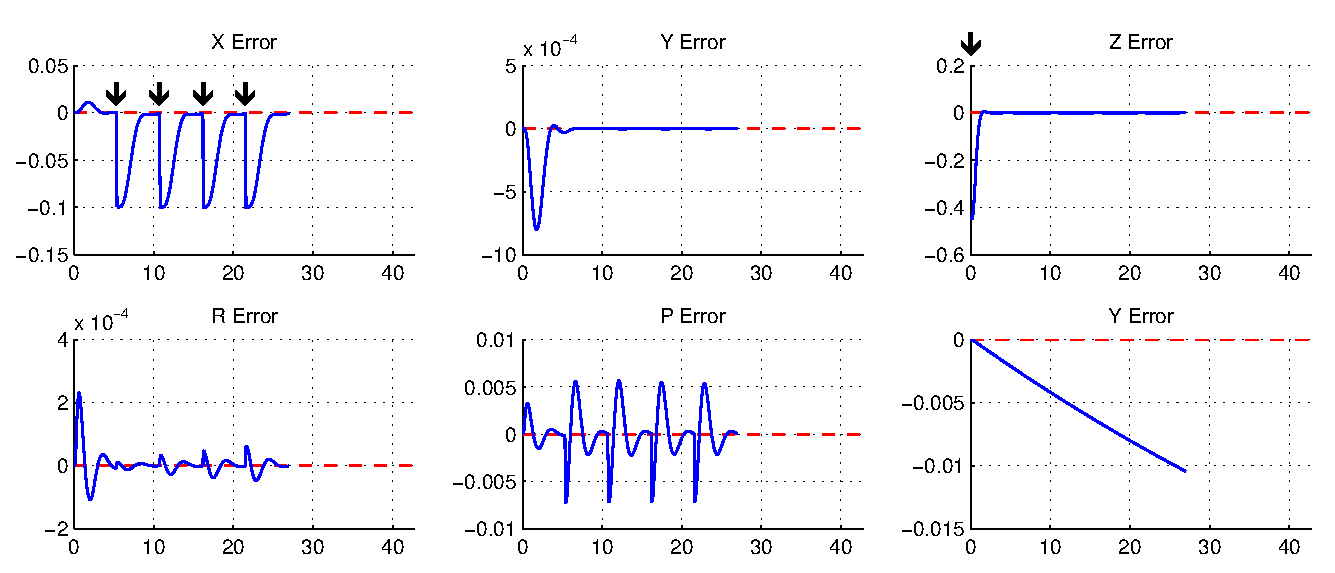
\includegraphics[width = 0.75\textwidth]{normal.eps}\label{2normal}} \\
	\subfloat[][Behavior with Doubled {\tt Kp}]{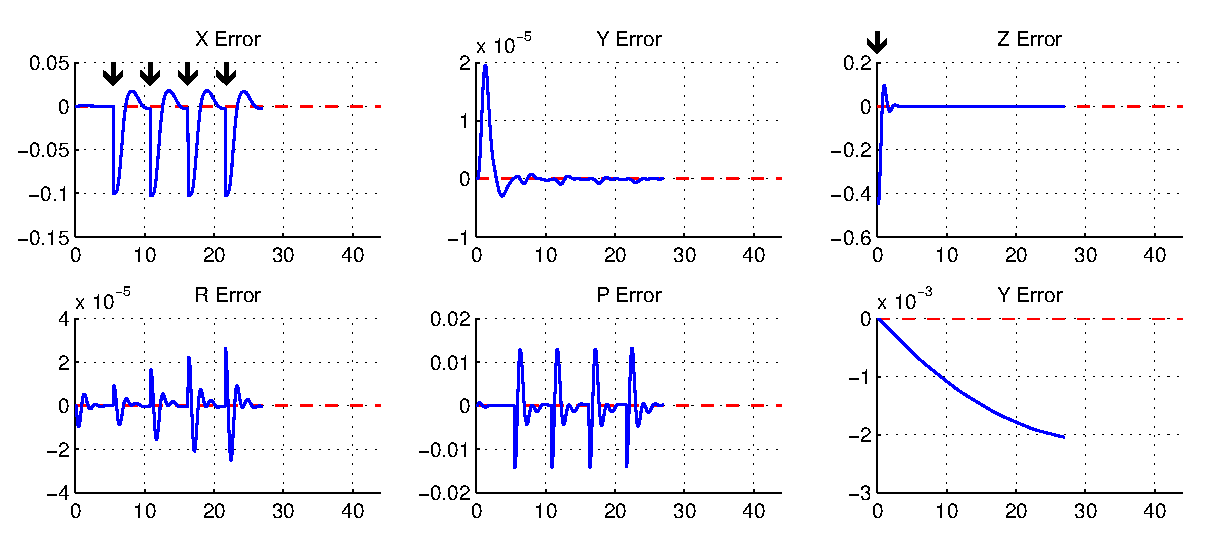
\includegraphics[width = 0.75\textwidth]{doublekp.eps}\label{2doublekp}}\\
	\subfloat[][Behavior with Doubled {\tt Kd}]{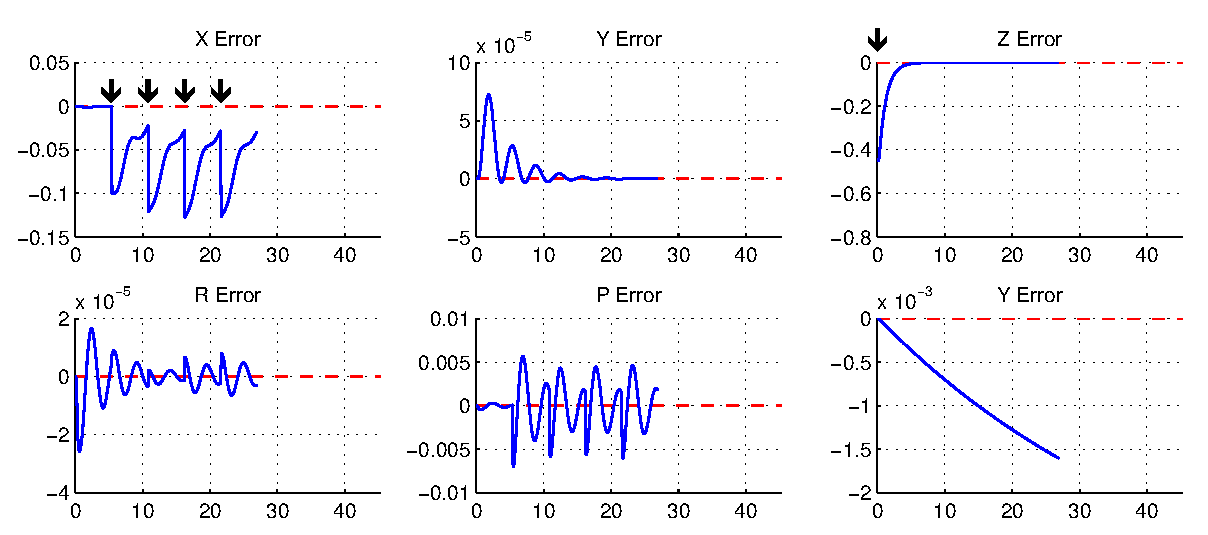
\includegraphics[width = 0.75\textwidth]{doublekd.eps}\label{2doublekd}}
	\caption{Position and Attitude (versus time [second]) with Different Gains}
		{\it New waypoints are sent to the system at points indicated by arrows.}
\end{figure}

The system oscillates between waypoints through a slight overshoot reaction.
The system then converges to the desired position in a short amount of time (within two oscillation cycles).
Modifying the gains associated with position control and attitude control
will change the oscillation behavior of the system. Specifically,
tuning the {\tt Kp} gains will increase the oscillation of the system,
while changing the {\tt Kd} gains will damp the oscillation behavior, at the cost of slower system response.

After tuning for quick response time and stability,
we arrived at a set of gains that resulted in Figure \ref{2normal}.
The position of the system converges within one second and within
two oscillation cycles to the desired values. The roll and pitch of the
system are intentionally tuned for quick response. The quick response
allows the system to react immediately to any error even though oscillations
are often coupled with quick response time.

To observe the effects of modifying {\tt Kp} and {\tt Kd} gains,
we simply doubled each gain and plotted the results. Figure \ref{2doublekp} shows the
oscillating effects from doubling {\tt Kp} values for both position control
and attitude control. More severe overshoots and oscillations in most
fields resulted from higher {\tt Kp} gains. Doubling {\tt Kd} gains smoothed out the
responses while adding a slight delay to the response time, as shown in Figure \ref{2doublekd}.
Due to this delay, the $x$-position is lagging behind the desired value.

\section{Line-Tracking Performance}

To develop the line tracking controller, we produced desired position and velocity
profiles for the system to follow. Each profile contains 300 waypoints. In our implementation,
the system will take off, fly to a height of one meter in the $z$-direction, hover,
and return to the ground. The velocity profile resembles a hill with a flat top.
The system will accelerate to a fixed speed, remain at the desired speed, and decelerate
as it approaches the final desired position. The tracking reference is updated to the next
waypoint when the position error measurement - in Euclidean distance - is within a defined
threshold of one centimeter.

The system $z$-value shows significant oscillations about the waypoints,
as shown in Figure \ref{errortuned}. This effect is caused by the alternating acceleration
and deceleration of the system as it closes in at the waypoint before the target
reference position is updated to the next waypoint. The position and velocity profiles
and the odometer measurements are shown in Figure \ref{posveltuned}. The tracking performance is
perceivably satisfying. Noise is observed near the initial movements of the system,
but this effect is expected as the system accelerates from the resting position.

\begin{figure}[h!]
	\centering
	\subfloat[][Normals Gains]{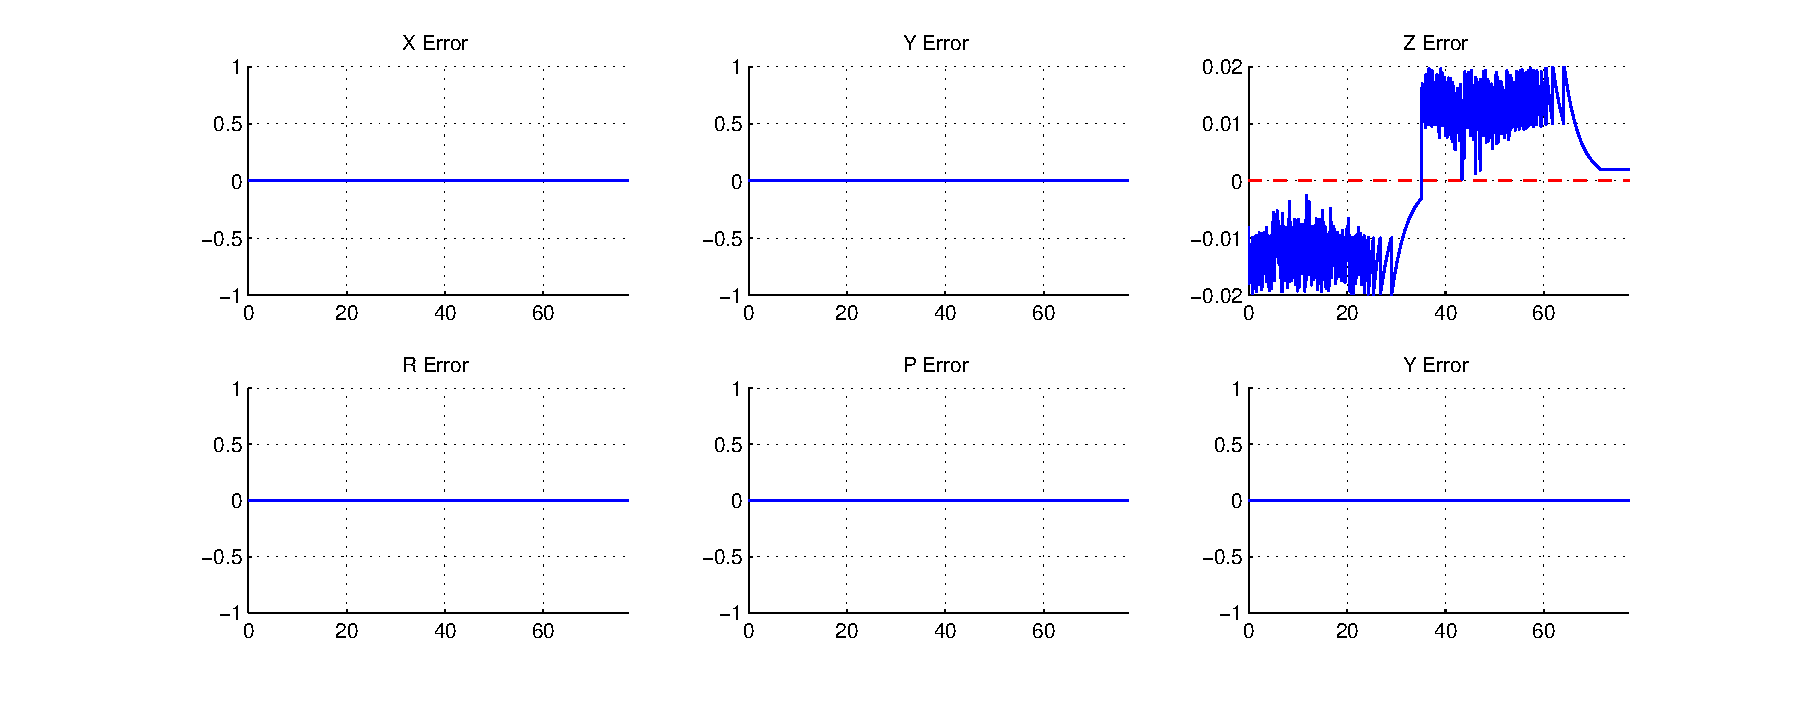
\includegraphics[width = 0.9\textwidth]{error_tuned.eps}\label{errortuned}} \\
	\subfloat[][Doubled {\tt Kp}]{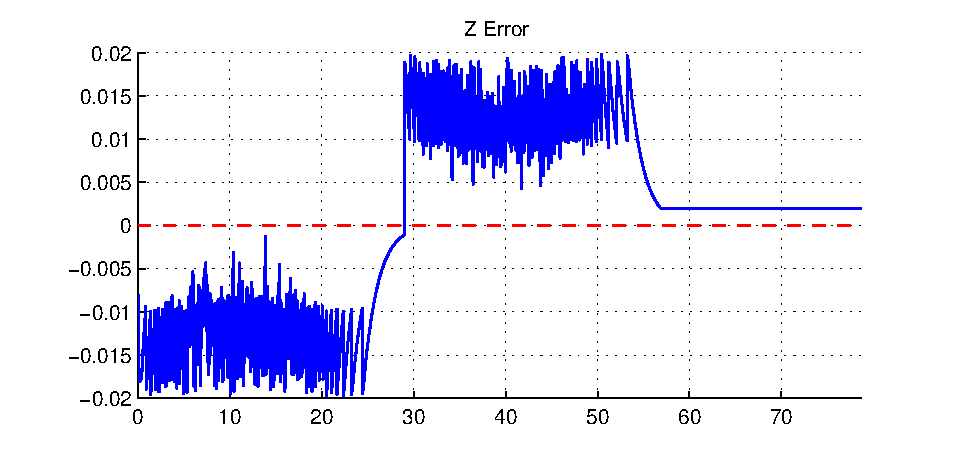
\includegraphics[width = 0.45\textwidth]{error_tuned2xkp.eps}\label{errortuned2xkp}}
	\subfloat[][Doubled {\tt Kd}]{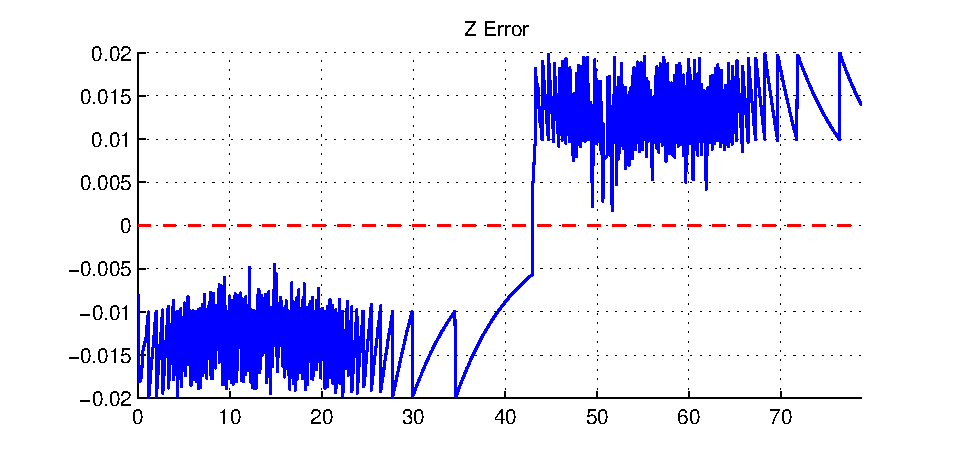
\includegraphics[width = 0.45\textwidth]{error_tuned2xkd.eps}\label{errortuned2xkd}} 
	\caption{Errors with Different Sets of Gains}  {\it Errors on x, y, roll, pitch, yaw remain the same for different gains.}
\end{figure}

Modifying the gains associated with the position control (outer loop)
changes the oscillation behavior of the system. The general behaviors of tuning {\tt Kp} and {\tt Kd}
 remain the same as described in the second question. One note is that, for this problem, we increased
 {\tt Kd} value and lowered the {\tt Kp} value in the $z$-direction to allow our controller to 
track the velocity closely. In another word, the increase in {\tt Kd} value added more weights on velocity in our controller.

To observe the effects of modifying {\tt Kp} and {\tt Kd} gains, we simply doubled each gain and plotted
the results. Figure \ref{errortuned2xkp} shows the oscillating effects from doubling {\tt Kp} values
for the position control. By doubling {\tt Kp} values, the velocity tracking error increases.
The increase in {\tt Kp} values shifts the weights from velocity tracking towards position tracking
in our controller. Doubling {\tt Kd} gains allowed the controller to track the velocity more closely,
at the cost of slower response to converge to the desired position, as shown in Figure \ref{errortuned2xkd}.
The tracking performances for position and velocity for doubling {\tt Kp} values and {\tt Kd} values are
shown in Figure \ref{posveltuned2xkp} and Figure \ref{posveltuned2xkd}, respectively. The system tracks the position and velocity closely.
Noise is again observed near the initial movements of the system.

\begin{figure}[h!]
	\centering
	\subfloat[][Normal Gains]{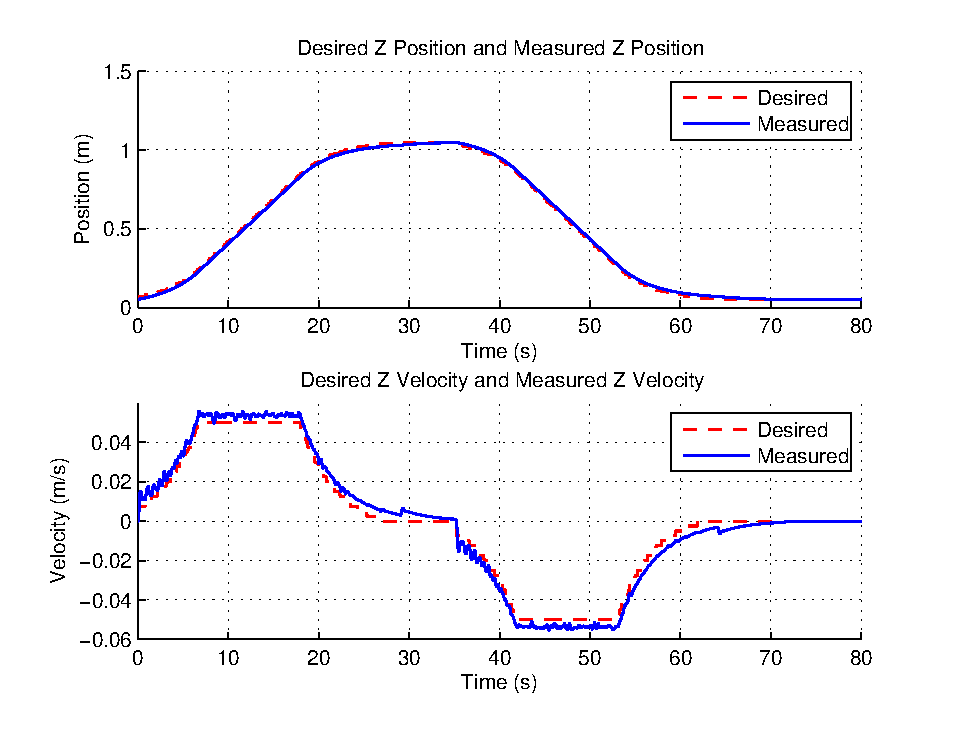
\includegraphics[width = 0.5\textwidth]{pos_vel_tuned.eps}\label{posveltuned}}
	\subfloat[][Doubled {\tt Kp}]{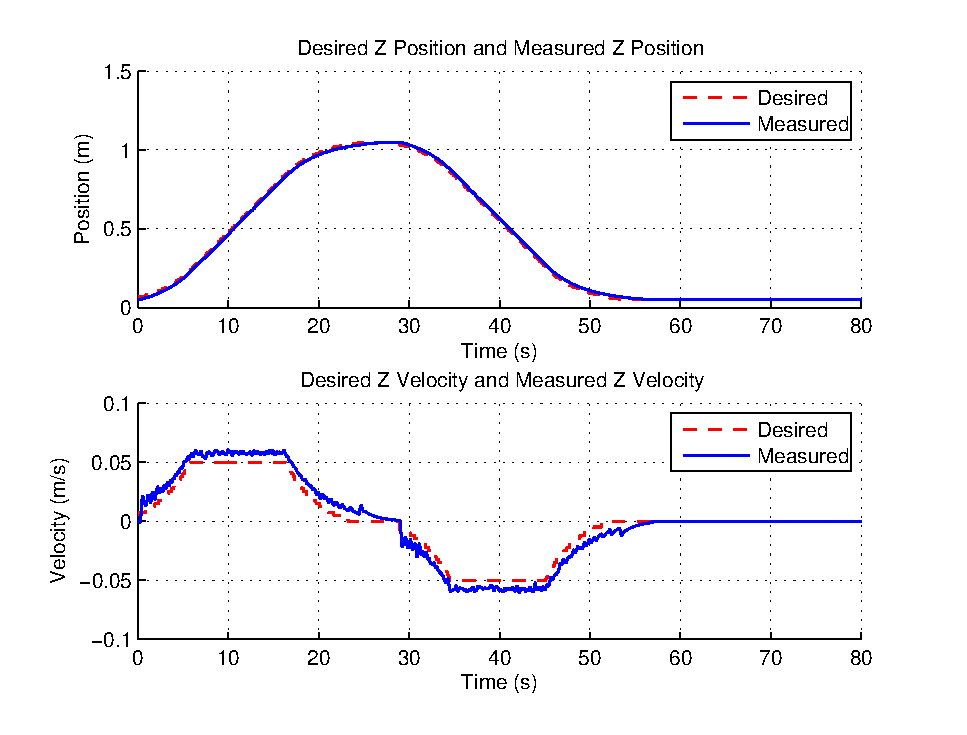
\includegraphics[width = 0.5\textwidth]{pos_vel_tuned2xkp.eps}\label{posveltuned2xkp}}	 \\
	\subfloat[][Doubled {\tt Kd}]{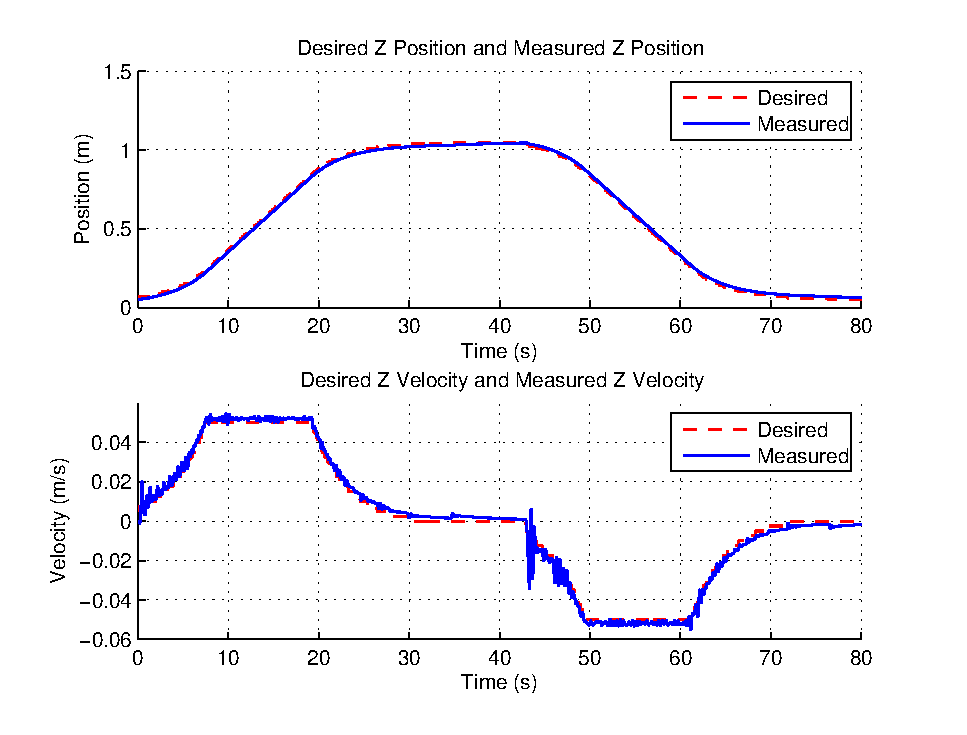
\includegraphics[width = 0.5\textwidth]{pos_vel_tuned2xkd.eps}\label{posveltuned2xkd}}
	\caption{Carefully Tuned Gains Yield Optimum Performance}
\end{figure}


\vfill
\begin{center}
	
\includegraphics[scale = 0.4]{evolutus-black.eps}
\end{center}

\thispagestyle{fancy}
	
\end{onehalfspacing}
\end{document} 